\lecture{22}{Average Values and the Equipartition Theorem}{Qiang Zhu}{scribe-name1,2,3}
%\footnotetext{These notes are partially based on those of Nigel Mansell.}
% **** YOUR NOTES GO HERE:
% Some general latex examples and examples making use of the
% macros follow.  
%**** IN GENERAL, BE BRIEF. LONG SCRIBE NOTES, NO MATTER HOW WELL WRITTEN,
%**** ARE NEVER READ BY ANYBODY.

\section{Average Values}
In the previous section, we saw how to calculate the probability that a system is in any particular one of its
microstates in equilibrium with a reservoir at $T$. In the statistical mechanical systems that we are considering,
each probability is given by 
\begin{equation}
\bar{E} = \frac{1}{Z} \sum_s E(s)e^{-\beta E(s)}
\end{equation}

Similarly, the average value of any other variable of interest can be computed in the same way.
\begin{equation}
\bar{X} = \frac{1}{Z} \sum_s X(s)e^{-\beta E(s)}
\end{equation}

By using this equation, we will get the average value of any property. In statistical mechanics, we shall also
understand the fluctuations.

A very nice feature of the partition function is that 
\begin{equation}
\bar{E} = -\frac{1}{Z} \frac{\partial{Z}}{\partial{\beta}} = -\frac{\partial{\text{ln}Z}}{\partial {\beta}}
\end{equation}
when $\beta$ = 1/$kT$. These formulas can be extremely useful when you have an explicit formula for $Z$
\begin{equation}
\bar{E^2} = \frac{1}{Z} \frac{\partial^2{Z}}{\partial{\beta^2}} 
\end{equation}


\section{Rotation of Diatomic Molecules}
For a diatomic molecule, its rotational energies are quantized. The allowed rotational energies are,
\begin{equation}
E(j) = j(j+1)\epsilon
\end{equation}

where $j$ can be 0, 1, 2, etc, and $\epsilon$ is a constant that is inversely proportional to the molecule's moment of inertia.
The number of degenerate states for level $j$ is 2$j$+1. Given the energy level, we can write the partition function as a sum over $j$,
\begin{equation}
Z_\text{rot} = \sum_{j=0}^{\infty} (2j+1)e^{-E(j)/kT} = \sum_{j=0}^{\infty}(2j+1) e^{-j(j+1) \epsilon /kT}
\end{equation}
 
Unfortunately, there is no way to evaluate the sum exactly in closed form. But it is not hard to do it numerically. Even better,
we can approximate the sum as an integral that yields a very simple result.

\begin{figure}[h]
\centering
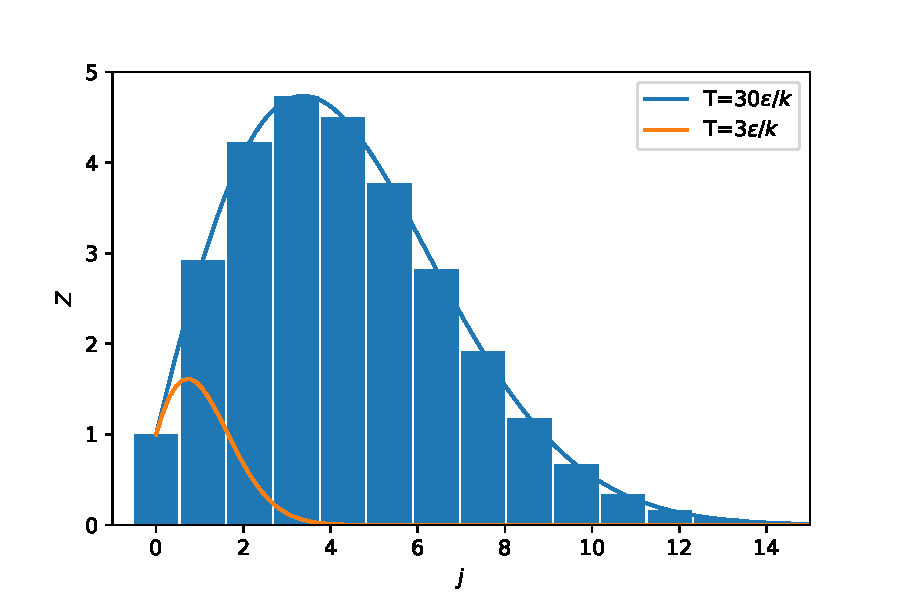
\includegraphics[width=10cm]{imgs/Rotation}
\caption{The partition sum for two different temperatures. }
\end{figure}

If we draw the curve, we could clearly see that the partition function is approximately the area under this curve at high $T$
\begin{equation}
Z_\text{rot} \approx \int_{0}^{\infty}(2j+1) e^{-j(j+1) \epsilon /kT} dj = \frac{kT}{\epsilon}  ~~~~~~~~(\text{when} ~kT >> \epsilon)
\end{equation}
 
As expected, the partition function increases when $T$ increases. For CO at room $T$, $Z_\text{rot}$ is slightly greater than 100.

With such approximation, we can then calculate the energy as well,
\begin{equation}
\bar{E}_\text{rot} = -\frac{1}{Z} \frac{\partial Z}{\partial {\beta}} 
                   = -(\beta\epsilon) \frac{\partial(1/\beta\epsilon)}{\partial{\beta}}=1/kT
\end{equation}
 
This is just the prediction of the equipartition theorem, since a diatomic molecule has two rotational degrees of freedom. 
At low temperature, the 3rd law tells us that the heat capacity must go to zero.
Above is the case of diatomic molecules made of different atoms. If it is N$_2$, 
\begin{equation}
Z_\text{rot} \approx \frac{kT}{2\epsilon}
\end{equation}
 
But this won't effect the energy and heat capacities. (problem 6.30)


\section{Equipartition Theorem}
The equipartition theorem has been extensively used in this class. However, we haven't proved it yet.
It turns out that the proof is quite easy, with the help of Boltzmann factors.

Suppose any energy term is in quadratic form, namely,
\begin{equation}
E(q) = cq^2
\end{equation}

The partition function is
\begin{equation}
Z = \sum_q e^{-\beta E(q)} = \sum_q e^{-\beta cq^2}
\end{equation}

Again, we can transform the sum to an integral
\begin{equation}
Z = \frac{1}{\Delta{q}} \int_{-\infty}^{\infty}  e^{-\beta cq^2} dq
\end{equation}

Let $x=\sqrt{\beta c}q$, so 

\begin{equation}
Z = \frac{1}{\Delta{q}\sqrt{\beta c}}\int_{-\infty}^{\infty}  e^{-x^2} dx
\end{equation}

The function $e^{-x^2}$ is called a Gaussian function.
\begin{equation}
\int_{-\infty}^{\infty}  e^{-x^2} dx = \sqrt{\pi}
\end{equation}

Therefore,
\begin{equation}
Z = \frac{1}{\Delta{q}} \sqrt{\frac{\pi}{\beta c}} = C\beta^{-1/2}
\end{equation}
where $C=\sqrt{\pi/c}/\Delta{q}$

and the energy can be readily computed,
\begin{equation}
\bar{E} = -\frac{1}{Z} \frac{\partial Z}{\partial {\beta}} = ~~~~~~~~~~~~~~~~~~~~~~~~~~~~ = \frac{1}{2}kT
\end{equation}

The limitation of the theorem is that we actually used the integral to replace the sum, which is correct when the spacing between energy level ($\epsilon$) is much less than $kT$.


